\subsection{Komponenten}

In diesem Kapitel werden die Komponenten des Volksbots und die Gesamtstruktur  durch eine Architekturdarstellung beschrieben. Bei dem Volksbot handelt es sich um einen modular aufgebauten und mobilen Roboter, der vom Frauenhofer-Institut IAIS entwickelt wurde. Die in diesem Projekt verwendeten Prototypen bestehen aus drei zentralen Elementen. 

	\begin{figure}[h!]
		\centering
			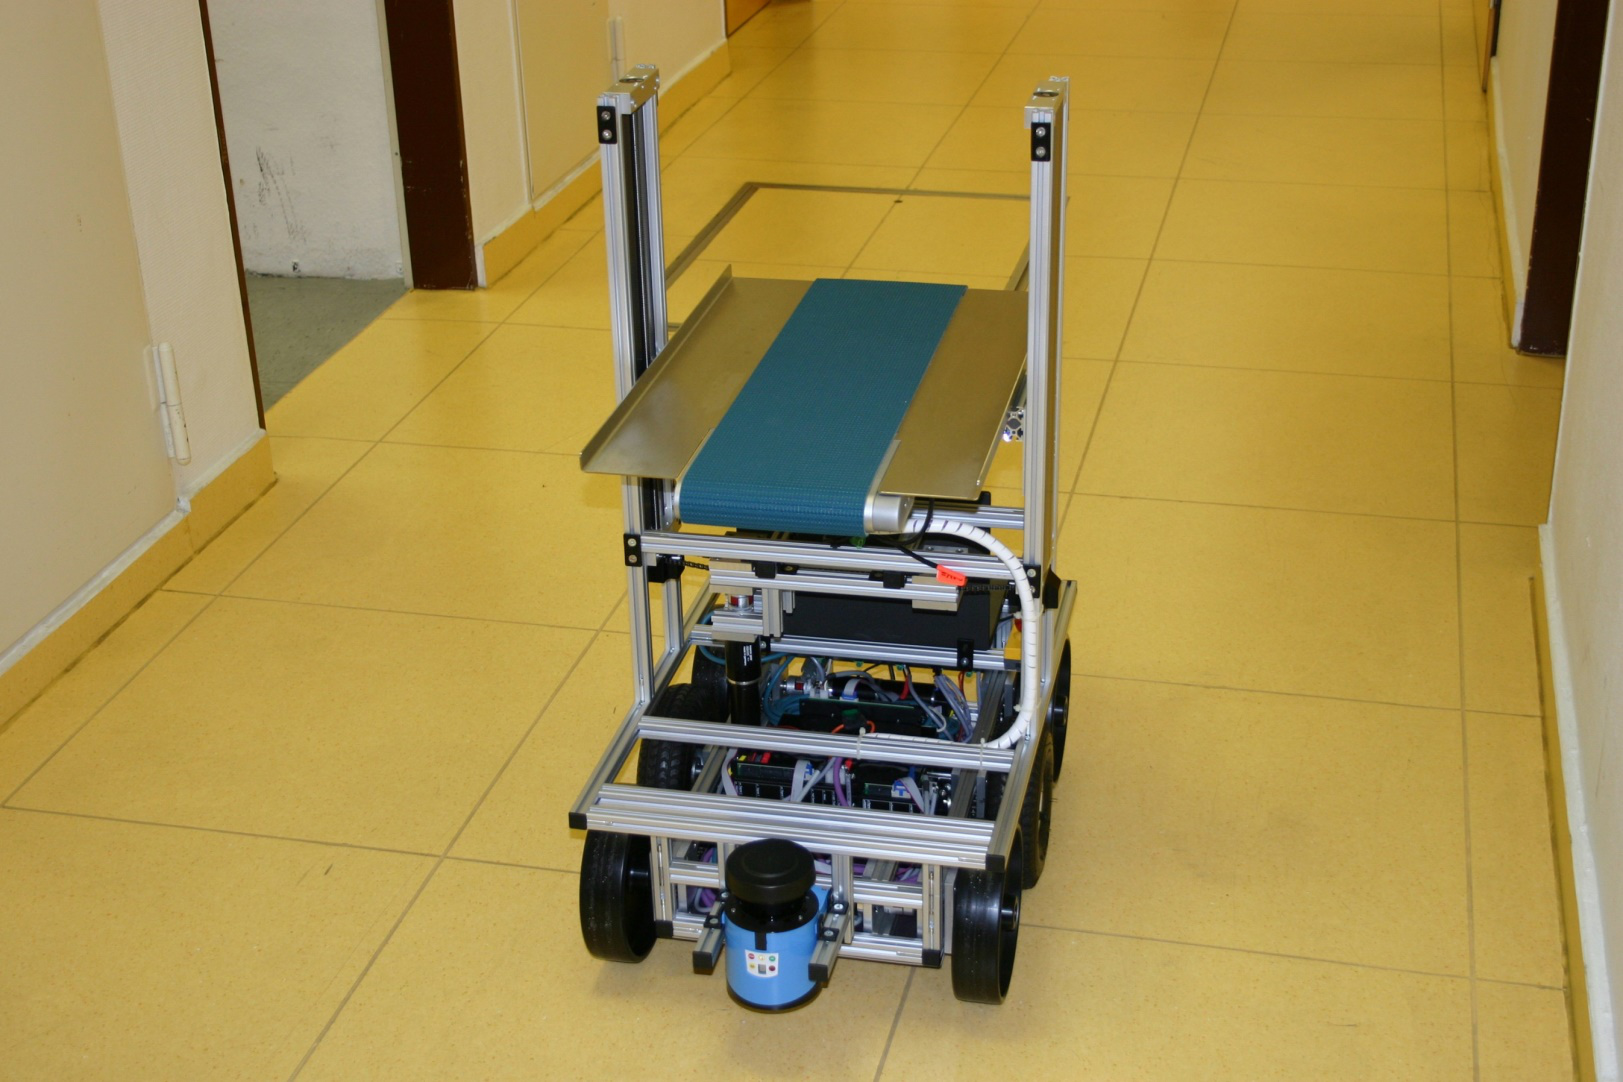
\includegraphics[width=0.9\textwidth]{drive/Volksbot.png}
			\caption{Darsellung eines Volksbots}
			\label{Volksbot}
	\end{figure}	




\subsubsection{Fahreinheit}

Die Fahreinheit wird aus zwei Maxonantrieben links und rechts, sowie dem Gerüst des Bots gebildet. Vorne befindet sich ein SICK LMS100 Laserscanner,  hinten ein SICK TiM310 Laserscanner. Angesteuert werden die Hardwarekomponenten mit Hilfe von vier Epos2 Controllern, die mit Hilfe einer CAN-Verbindung ansteuerbar sind. 

\subsubsection{Hub-Förderband}

Zum Transportieren der Pakete ist der Volksbot mit einer Hubeinheit ausgestattet, die zum Schutz vor Überdrehungen zwei Hallsensor auf beiden seiten beinhaltet. Des weiteren befindet sich auf der Hubeinheit ein Förderband, an dem sich zwei Lichtschranken befinden. Diese sollen zur Ermittlung des Beladungszustandes dienen. 

\subsubsection{Steuereinheit}

Gesteuert wird das System mit Hilfe eines Notebooks, welches unter Ubuntu mit Hilfe des Robot Operating System (ROS) die Hardware anspricht. Auf dem Notebook werden ausserdem sämtliche 
Berechnungen durchgeführt. Neben der Ansteuerung der EPOS2 Controller wird der SICK LMS100 über eine Ethernet Schnittstelle angeschlossen. Zur Kommunikation mit den Rampen wird zusätzlich ein MICAZ Modul verwendet, welches mittels einer USB Schnittstelle mit dem Notebook verbunden ist.

\subsubsection{Architektur}

Der systematische Aufbau des Volksbots ist in Abbildung \ref{fig:architecture_volksbot} dargestellt. Die Funktionen des Roboters basieren auf der Auswertung und Ansteuerung der Sensoren bzw. Aktoren. Alle Operationen, wie z.B. die Lokalisation, die Routenplanung, der Vorgang der Paketübergabe, laufen auf dem Robot Operating System und nutzen die Daten der Sensorik zur geeigneten Ansteuerung der Aktoren. Gesteuert werden die Operationen über die externe Kommunikationsebene, welche aus einem MICAz-Modul besteht. Hier werden Aufträge empfangen und auf der Operationsebene in zugehörige Ziele übersetzt.

\begin{figure}[h!]
 \centering
		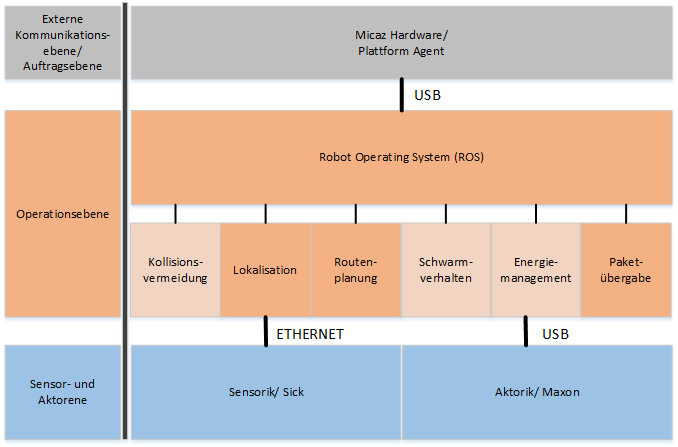
\includegraphics[width=1\textwidth]{drive/DRIVE_Architektur.png}
	\caption{Architektur des Volksbot}
	\label{fig:architecture_volksbot}
\end{figure}

Funktionen, die in dunklem orange hervorgehoben sind, deuten deren existenzielle Wichtigkeit an und geben ein erstes Anzeichen darauf, welche Funktionen erfolgreich umgesetzt werden konnten.